\documentclass[../main.tex]{subfiles}

\begin{document}

 \subsubsection{Centro de rigidez}

 Se puede determinar mediante ecuaciones tales como:

 \begin{align*}
   y_{cr} &= \frac{\Sigma K_{xi} * y_i}{\Sigma K_{xi}} \\[5pt]
   x_{cr} &= \frac{\Sigma K_{yi} * x_i}{\Sigma K_{yi}}
 .\end{align*}

La importancia de este punto es que debemos intentar hacer coincidir la 
resultante de las cargas con este punto.

Además, podemos obtener los momentos de primer orden de rigideces como:

\begin{align*}
  S_x &= \Sigma K_{xi} * X_{cr} \\[5pt]
  S_{y} &=  \Sigma K_{yi} * Y_{cr} 
.\end{align*}

\subsubsection{Movimiento oblicuo}

Si se diera que no coinciden el centro de rigidez con la recta de acción de la
fuerza horizontal exterior, se produce una excentricidad que da lugar a la 
aparición de un momento torsor que provocará una rotación. 

En el caso general, las fuerzas horizontales de planta provocan esfuerzos de
corte, que se descompone en dos direcciones y un momento torsor. Se produce
un desplazamiento, medido como $\delta_x$, $\delta_y$ y un rotación $\phi$.

\begin{figure}[htpb]
  \centering
  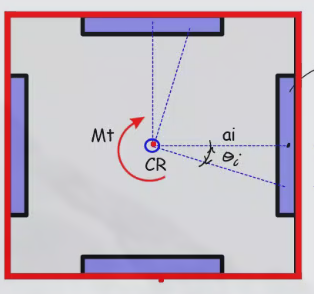
\includegraphics[width=0.45\textwidth]{../images/20210601/oblicuo}
  \caption{Esquema.}
  \label{fig:oblicuo}
\end{figure}

De esto podemos ver que el corrimiento será:
\begin{align*}
  Q_i = K_i * \Delta_i \hspace{0.25cm} \xrightarrow{\hspace*{0.5cm}} \hspace{0.1cm} Q_i = \frac{\theta_i}{K_i}
.\end{align*}

Donde en este caso, podemos distinguir, desde la imagen, que:
\begin{align*}
  \Delta_i &= \theta_i * a_i \\[5pt]
  \theta_i &= \frac{\Delta_i}{a_i}
.\end{align*}

Reemplazando las dos ecuaciones anteriores, podemos llegar a lo siguiente:
\begin{align*}
  \theta = \theta_i = \frac{\Delta_i}{a_i} = \frac{\theta_i}{k_i*a_i}
.\end{align*}

Por otro lado, sabemos que:

\begin{align*}
  Q_i &= K_i * \Delta_i = K_i * \theta * a_i \\[5pt]
  M_i &= Q_i * a_i = K_i * \theta * a_i²
.\end{align*}

Planteando equilibrio de momentos en el centro de rigidez:

\begin{align*}
  M_t &= \Sigma M_i = \Sigma K_i * a_i² * \theta \\[5pt] 
  \theta &= \frac{M_t}{\Sigma K_i * a_i²}
.\end{align*}

Igualando las dos expresiones de $\theta$, podemos despejar:

 \begin{align*}
   \frac{M_t}{\Sigma K_i * a_i²} &= \frac{Q_i}{K_i * a_i} \\[5pt]
   Q_i = M_t * \frac{k_i*a_i}{\Sigma k_i * a_i²} &= M_t = \frac{K_i * a_i}{J_r}
.\end{align*}

Donde $J_r$ es un momento polar de las rigideces.

\subsubsection{Análisis de casos}

En un sistema conformado solamente por tabiques, es posible la utilización de
las formulas encontradas anteriormente (y también dadas en las diapositivas
del profesor).

Si el sistema se compone de dos subestructuras verticales, el problema es 
isostático, y la distribución de cargas depende únicamente de su ubicación.

\subsection{Método de análisis tridimensional de estructuras}

La distribución de fuerzas dinámicas debido a acciones dinámicas puede ser
resuelto mediante métodos iterativos o elementos finitos. Lo más frecuente
es recurrir a los primeros, reservando la segunda para casos muy particulares. 

\subsubsection{Estructura y sub-estructura}

Denominamos \textbf{estructura} de un edificio al esqueleto resistente del
mismo, destinada a transferir las diversas cargas a la fundación.

Para su análisis, se la descompone en \textbf{sub-estructuras}, contenidas
en planos verticales y horizontales. Dentro de estas, podemos considerar
los planos correspondientes a pisos o techos de edificio, que además de
resistir fuerzas verticales de peso propio y sobrecarga, también soporten 
fuerzas horizontales y las trasmitan a las subestructuras verticales vinculadas
a las mismas.

\subsubsection{Análisis de movimiento plano}

Un edificio tiene un \textbf{movimiento plano} cuando todos las subestructuras
horizontales poseen un movimiento de traslación paralelo a una misma dirección.
En este caso se considera que los pisos no rotan, y solo se desplazan un
valor $u_i$. 

Si consideramos $f_i$ la fuerza exterior aplicada en el nivel $i$, que se 
une en un vector  $f = \{f_1, f_2,\ldots, f_n\}$. Los desplazamientos en cada
planta también serán $u=\{u_1,u_2,\ldots,u_n\}$. Podemos considerar conocida
la matriz de rigidez de la subestructura, que denominamos $K_p$, y consideramos
por último las fuerzas $f_p$ que reúne las fuerzas exteriores sobre $p$. 

De lo conocido de Análisis Estructural I, podemos desarrollar las siguientes
ecuaciones matriciales:

\begin{align*}
  f &= k_i * u_i \\[5pt]
  u &= k_i^{-1} * f
.\end{align*}

Esto nos permite la determinación de los desplazamientos.


\begin{figure}[htpb]
  \centering
  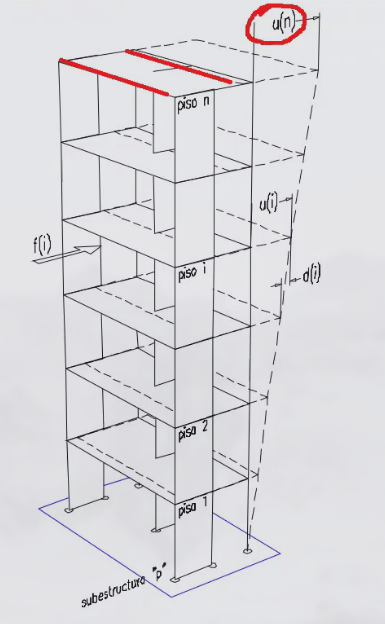
\includegraphics[width=0.5\textwidth]{../images/20210601/movplano}
  \caption{Estructura con movimiento plano}
  \label{fig:movplano}
\end{figure}

\subsubsection{Análisis de movimiento oblicuo}





\end{document}
